\documentclass{standalone}
\usepackage{amsmath}
\usepackage{tikz}
\usetikzlibrary{shapes.geometric, arrows}

\begin{document}
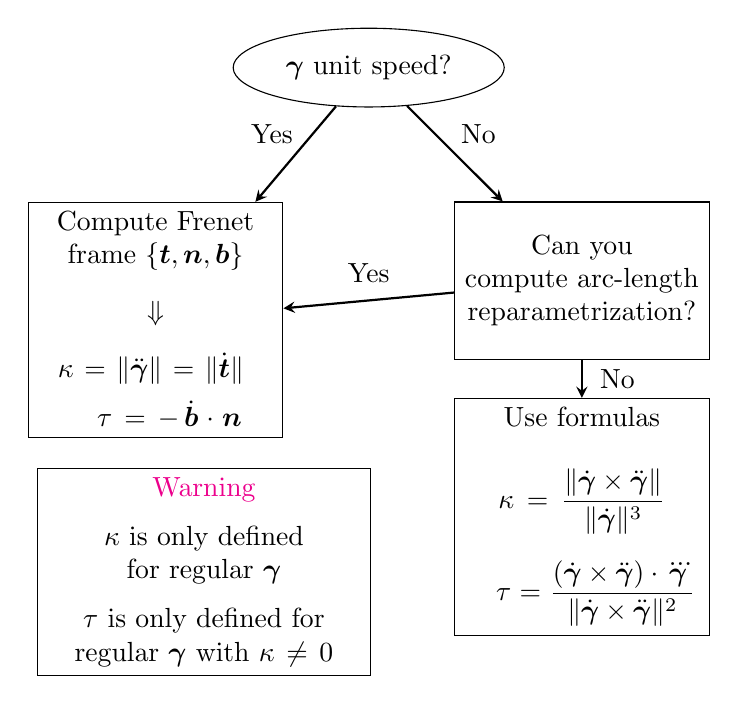
\begin{tikzpicture}
    % Define styles for blocks and arrows
    \tikzstyle{topblock} = [ellipse, draw, text centered, text width=2.2cm, minimum height=1cm]
    \tikzstyle{rectblock} = [rectangle, draw, text centered, text width=3cm, minimum height=2cm]
    \tikzstyle{rectblocklarge} = [rectangle, draw, text centered, text width=4cm, minimum height=2cm]
    \tikzstyle{arrow} = [thick,->,>=stealth]

    % Nodes
    \node (gamma) [topblock] {$\boldsymbol \gamma$ unit speed?};
    \node (yes) [rectblock, below left of=gamma, xshift=-2cm, yshift = -2.5cm] {Compute Frenet frame $\{ {\boldsymbol{t}}, \boldsymbol{n},\boldsymbol{b} \}$ \\  \vspace{0.3cm} $\Downarrow$  \\ \vspace{0.3cm} $\kappa =  \| \ddot{\boldsymbol{\gamma}} \| =  \| \dot{\boldsymbol{t}}  \| $ \vspace{0.1cm} \\  \vspace{0.1cm} $\quad\tau = - \, \dot{ \boldsymbol{b} } \cdot \boldsymbol{n}$};
    \node (no) [rectblock, below right of=gamma, xshift=2cm, yshift = -2cm] {Can you \\compute arc-length reparametrization?};
	
	\node (formulas) [rectblock, below right of=gamma, xshift=2cm, yshift = -5.0cm] {Use formulas  \\  \vspace{0.5cm}  $\kappa = \dfrac{ \| \dot{\boldsymbol{\gamma}}  \times \ddot{\boldsymbol{\gamma}} \|  }{  \| \dot{\boldsymbol{\gamma}}  \|^3 } $ \\ \vspace{0.3cm} $\,\,\,\,\,\,\tau = \dfrac{( \dot{\boldsymbol{\gamma}}  \times \ddot{\boldsymbol{\gamma}} ) \cdot \dddot{ \boldsymbol{\gamma} } }{ \| \dot{\boldsymbol{\gamma}}  \times \ddot{\boldsymbol{\gamma}} \|^2  }$}; 
	
	\node (warning) [rectblocklarge, below right of=gamma, xshift=-2.8cm, yshift = -5.7cm] {\textcolor{magenta}{Warning} \\ \vspace{0.2cm} $\kappa$ is only defined for regular $\boldsymbol{\gamma}$ \\ \vspace{0.2cm} $\tau$ is only defined for regular $\boldsymbol{\gamma}$ with $\kappa \neq 0$};
	

    % Arrows
    \draw [arrow] (gamma) -- (yes) node[midway, above, xshift=-0.3cm, yshift = 0cm] {Yes};
    \draw [arrow] (gamma) -- (no) node[midway, above, xshift=0.3cm, yshift = 0cm] {No};
    \draw [arrow] (no) -- (yes) node[midway, above, xshift=0cm, yshift = 0.1cm] {Yes};
    \draw [arrow] (no) -- (formulas) node[midway, right, xshift=0.1cm, yshift = 0cm] {No};

\end{tikzpicture}

\end{document}